\documentclass[conference]{IEEEtran}
\IEEEoverridecommandlockouts
\usepackage{cite}
\usepackage{amsmath,amssymb}
\usepackage{algorithmic}
\usepackage{graphicx}
\usepackage{textcomp}
\usepackage{booktabs}
\usepackage{url}
\usepackage[hidelinks]{hyperref}
\def\BibTeX{{\rm B\kern-.05em{\sc i\kern-.025em b}\kern-.08em T\kern-.1667em\lower.7ex\hbox{E}\kern-.125emX}}

\begin{document}

\title{Evidence-Based Multi-Layer Authorization for\\ Voice Assistants: Calibrated Fusion and\\ Cost-Derived Decision Thresholds}

\author{\IEEEauthorblockN{Atharva Kadge, Damodar Kamath, Shlok Kanvinde}
\IEEEauthorblockA{\textit{Department of Computer Engineering} \\
\textit{Sardar Patel Institute of Technology}\\
Mumbai, India}}

\maketitle

\begin{abstract}
Voice assistants increasingly authorize payments and control physical devices,
yet most deployed systems verify the speaker once, compare a similarity score
against a hand-chosen cutoff, and treat every request as equally consequential.
This paper presents SecureVoice, an authorization architecture that replaces
hand-tuned score cutoffs with two principled mechanisms: per-layer probability
calibration, which converts heterogeneous detector outputs into additive
log-likelihood ratios, and a decision threshold derived from Bayes risk
minimization, which rises logarithmically with the stake of the request. Four
independent evidence layers---speaker verification, replay liveness,
synthetic-speech detection, and a contextual layer that inspects the spoken
command itself---feed a policy layer that returns allow, challenge, or deny.
We report three findings from measurement rather than assertion. First, the
customary naive-Bayes summation of layer scores is invalid in this setting
because the layers test different hypotheses: an impostor speaking live is
correctly reported as human by the anti-spoofing layer, and that correct
statement cancels the correct rejection from the speaker layer, raising
impostor false acceptance from 0.25\% to 52.25\%. Replacing summation with a
conjunctive weakest-link rule removes the effect and guarantees that adding a
layer can never open a hole. Second, a layer ablation shows every layer is
necessary and none is redundant: removing liveness raises replay false
acceptance from 1.25\% to 74.0\%, removing anti-spoofing raises clone false
acceptance to 43.25\%, and removing the contextual layer raises prompt-injection
false acceptance from 10.0\% to 23.5\%. Third, a sensitivity sweep localizes the
policy's dependence on its assumed constants almost entirely to the attack
prior, which is the one constant a deployment can estimate from its own logs.
We report all results with their scope, including two layers evaluated on small
or synthetic corpora, and we identify these explicitly as requiring
validation.
\end{abstract}

\begin{IEEEkeywords}
voice assistant security, speaker verification, anti-spoofing, replay
detection, score calibration, log-likelihood ratio, Bayes risk, decision cost
function, prompt injection
\end{IEEEkeywords}

\section{Introduction}

Voice has become a transactional interface. Assistants embedded in phones,
speakers, cars and appliances now place orders, move money and unlock doors,
and the number of voice-enabled devices continues to grow. The security
assumptions of these systems, however, were largely inherited from an era in
which a voice command played music or reported the weather. When the worst
outcome of a misrecognized command was an unwanted song, a permissive design
was reasonable. When the worst outcome is an unauthorized payment, it is not.

Three properties of current deployments are, in our view, the source of the
problem.

\emph{Authentication is a single event.} A user is verified once, at the start
of an interaction, and every subsequent command inherits that verification.
An attacker who gains access mid-session inherits it too.

\emph{Verification reduces to one number against one cutoff.} A speaker
verification model emits a similarity score, the score is compared against a
threshold, and the threshold is chosen by intuition or by tuning on a
convenient dataset. The Phase-2 design that preceded this work followed
exactly this pattern, with a cosine similarity of $0.75$ treated as genuine,
$0.85$ as a strong match, and below $0.50$ as an impostor. Nothing in that
scheme explains why $0.75$ rather than $0.70$, and nothing connects the cutoff
to what a wrong decision actually costs.

\emph{Every request is treated alike.} A command that dims a lamp and a command
that transfers a large sum are subjected to the same test. Where systems do
distinguish between them, they typically do so through a small number of
hand-drawn amount bands, which is a coarse approximation of a relationship that
is, as we show, smooth and derivable.

These three properties interact badly with the modern threat landscape.
Text-to-speech and voice-conversion systems now produce speech that speaker
verification models accept as genuine \cite{wu2015spoofing,todisco2019asvspoof}.
Replay attacks require no machine learning at all, only a recording and a
loudspeaker. And once an assistant is mediated by a large language model, an
attacker can address the model directly in speech, attempting to override its
instructions---a voice-borne instance of the prompt injection problem
documented in text-based LLM applications \cite{greshake2023injection}.

\subsection{Contributions}

This paper describes a system built to address those properties, and reports
what measurement showed. Our contributions are:

\begin{enumerate}
\item \textbf{Calibrated evidence in place of raw scores.} Each layer's native
output---a cosine similarity, a softmax probability, a normality product---is
mapped by logistic calibration onto a log-likelihood ratio, so that
heterogeneous detectors become directly comparable and combinable
(Section~\ref{sec:calibration}).

\item \textbf{A negative result on additive fusion.} Calibrated LLRs are
log-odds and therefore appear to justify summation. We show by measurement that
summation is invalid here because the layers answer different questions, and
that it degrades impostor detection from 0.25\% to 52.25\% false acceptance. We
adopt a conjunctive weakest-link rule with the property that additional layers
can only lower the fused score (Section~\ref{sec:fusion}).

\item \textbf{A threshold derived from cost, generalized beyond money.} The
decision boundary follows from Bayes risk minimization using a detection cost
function \cite{kinnunen2018tdcf}, and rises logarithmically with the stake of
the request. We generalize the monetary amount to a \emph{stake} so that
requests carrying no rupee figure, such as disclosing a one-time password, are
not assigned the lowest possible bar (Section~\ref{sec:policy}).

\item \textbf{A per-threat ablation over four layers and five threats},
demonstrating that each layer covers a threat the others structurally cannot
(Section~\ref{sec:ablation}).

\item \textbf{A sensitivity analysis of the assumed cost constants},
identifying which assumption the system's behavior actually depends on
(Section~\ref{sec:sensitivity}).
\end{enumerate}

\subsection{Scope and honesty of reporting}

Two of the four evidence layers rest on limited data, and we state this
wherever their numbers appear rather than only in a closing paragraph. The
liveness layer is fitted on 15 live/replay pairs from a single speaker, room
and playback device. The contextual layer is calibrated on a
template-generated command corpus, because no public corpus of labelled
adversarial voice-assistant commands exists. Results derived from these are
reported as indicative and are marked as requiring validation. No number in
this paper is estimated, extrapolated or assumed; every figure is produced by
a script in the accompanying implementation.

\section{Literature Survey}

\subsection{Speaker verification}
Modern text-independent speaker verification embeds an utterance into a fixed
vector and compares vectors by cosine similarity. ECAPA-TDNN
\cite{desplanques2020ecapa} refined the time-delay neural network family with
channel attention, multi-layer feature aggregation and squeeze-excitation, and
remains a strong and widely used baseline; we use the SpeechBrain
implementation \cite{ravanelli2021speechbrain} trained on VoxCeleb
\cite{nagrani2017voxceleb}. Such models are highly effective against the threat
they are designed for---a different human---and, importantly for this work,
offer no defence at all against an accurate synthetic copy of the enrolled
voice.

\subsection{Spoofing countermeasures}
The ASVspoof series established shared datasets and evaluation protocols for
spoofing countermeasures \cite{todisco2019asvspoof,wang2020asvspoof}. Logical
access attacks comprise text-to-speech and voice conversion; physical access
attacks comprise replay. Subsequent editions extended evaluation to compressed
and transmitted speech and to deepfake audio \cite{yamagishi2021asvspoof}. Early countermeasures used engineered spectral
features with generative classifiers; contemporary systems operate on the raw
waveform. AASIST \cite{jung2022aasist} applies a heterogeneous spectro-temporal
graph attention network to a SincNet front end \cite{ravanelli2018sincnet}, and
its lightweight variant reaches approximately 1\% equal error rate on the
ASVspoof 2019 logical access evaluation set with fewer than $10^5$ parameters.
Related end-to-end raw-waveform systems such as RawNet2 \cite{tak2021rawnet}
follow the same trend away from hand-engineered front ends.

A recurring and well-documented weakness is generalization. Countermeasures
trained on one corpus degrade substantially on unseen attacks and unseen
recording conditions \cite{muller2022generalize}. This is not a peripheral
caveat; it is the dominant practical obstacle, and we encountered it directly
(Section~\ref{sec:domaingap}).

\subsection{Liveness and replay detection}
Replay is the cheapest attack on a voice interface and requires no synthesis.
Detection exploits the fact that a replayed signal has passed through a
loudspeaker and a second acoustic path, which reshapes its spectral envelope.
Void \cite{ahmed2020void} demonstrated that lightweight spectral features
suffice for practical replay detection. A complementary line of work uses a
second physiological channel: bone conduction captured by a wearable is
present for genuine speech and absent for playback. That approach achieves high
accuracy but requires hardware that a smart speaker does not have, which is why
the present work pursues an air-conduction-only formulation. Vocal-tract-based
methods have also been used to separate genuine from synthetic speech
\cite{blue2022vocaltract}.

\subsection{Attacks on the assistant itself}
Beyond the acoustics of the speaker, the assistant is attackable as a system.
Inaudible ultrasonic carriers can inject commands a user cannot hear
\cite{zhang2017dolphin}. Adversarial perturbations can cause a speech
recognizer to transcribe an attacker's chosen text \cite{carlini2018audio}, and
speaker recognition systems are themselves susceptible to adversarial examples
\cite{chen2021bob}. Where a large language model interprets the command, the
model's instruction-following behaviour becomes an attack surface: an attacker
who controls part of the input can attempt to override the system prompt
\cite{greshake2023injection}. Surveys of voice assistant security consistently
observe that individual defences exist for individual threats, while integrated
frameworks do not \cite{cheng2022survey}.

\subsection{Calibration and cost-based decisions}
Detection scores are not probabilities, and comparing them across systems or
against a cost requires calibration. Platt scaling \cite{platt1999probabilistic}
fits a logistic map from score to posterior. In speaker recognition,
application-independent evaluation using calibrated log-likelihood ratios has
been standard for two decades \cite{brummer2006application}. The ASVspoof
challenges adopted a tandem detection cost function
\cite{kinnunen2018tdcf,kinnunen2020tandem} precisely because equal error rate
ignores the operational cost of the two error types. Our threshold derivation
follows directly from this literature; the contribution is its application to
an amount-dependent authorization decision, and its generalization beyond
monetary amounts.

\section{Research Gap and Problem Statement}

Table~\ref{tab:gap} summarizes the position. Each individual capability exists
in the literature and is mature. What does not exist, to our knowledge, is a
system that treats the outputs of several such capabilities as calibrated
evidence for different hypotheses, fuses them under a rule that is correct for
that structure, and compares the result against a threshold derived from the
consequences of the specific request.

\begin{table}[t]
\caption{Capabilities addressed in prior work and the integration gap}
\label{tab:gap}
\centering
\footnotesize
\begin{tabular}{@{}p{2.5cm}p{2.6cm}p{2.4cm}@{}}
\toprule
\textbf{Capability} & \textbf{Representative work} & \textbf{Status} \\
\midrule
Speaker verification & ECAPA-TDNN \cite{desplanques2020ecapa} & Mature \\
Synthetic detection & AASIST \cite{jung2022aasist} & Mature \\
Replay detection & Void \cite{ahmed2020void} & Mature \\
Prompt injection & \cite{greshake2023injection} & Emerging \\
Cost-based decisions & t-DCF \cite{kinnunen2018tdcf} & Mature \\
\midrule
\multicolumn{3}{@{}p{7.6cm}@{}}{\emph{Gap:} calibrated fusion of the above into
a single request-level authorization decision whose threshold is derived from
the stake of that request rather than chosen by hand.} \\
\bottomrule
\end{tabular}
\end{table}

\noindent\textbf{Problem statement.} Given a spoken request to a voice
assistant, decide whether to execute it, ask for further confirmation, or
refuse it, such that (i) each defensive component contributes evidence on a
common and interpretable scale, (ii) the combination rule is sound with respect
to the distinct hypotheses the components test, (iii) the decision boundary is
derived from the cost of being wrong about this particular request rather than
selected by hand, and (iv) every element of the resulting decision is
auditable.

\section{Proposed System and Methodology}

\subsection{Architecture}

SecureVoice is organized as four independent evidence sources and one decision
policy. We emphasize the distinction because it is frequently blurred: layers
1--4 are detectors that produce evidence; layer 5 is not a detector at all and
produces no score. It sets the bar and makes the call.

\begin{table}[t]
\caption{Layers, the question each answers, and the threat each covers}
\label{tab:layers}
\centering
\footnotesize
\begin{tabular}{@{}llp{2.5cm}@{}}
\toprule
\textbf{Layer} & \textbf{Question} & \textbf{Threat covered} \\
\midrule
L1 Voiceprint & Is this the enrolled user? & Impostor (different human) \\
L2 Liveness & Mouth or loudspeaker? & Replay of a recording \\
L3 Anti-spoofing & Human or synthesizer? & TTS / voice conversion \\
L4 Context & Is this request normal? & Coerced or manipulated request \\
\midrule
L5 Policy & \multicolumn{2}{l}{Sets $\tau$ from the stake; decides} \\
\bottomrule
\end{tabular}
\end{table}

The threat coverage in Table~\ref{tab:layers} is the substance of the layering
argument. It is not that more layers are safer in some general sense; it is
that each cell is a threat the other layers cannot see. An impostor is a real,
live human, so L2 and L3 correctly pass them. A synthetic clone of the enrolled
speaker is accepted by L1 precisely because the clone succeeded. A replayed
recording of the genuine user is the genuine user's voice and a genuine human
vocal tract, so both L1 and L3 pass it.

\subsection{Threat model}

We assume an attacker who can (i) speak near the device, (ii) obtain and replay
a recording of the enrolled user, (iii) synthesize the enrolled user's voice
from public samples using text-to-speech or voice conversion, and (iv) craft
the linguistic content of a command freely, including content addressed to any
language model in the pipeline. We assume the attacker cannot modify the
device's software, extract stored embeddings, or alter the audit log. Attacks
on the acoustic channel that bypass human hearing entirely, such as ultrasonic
injection \cite{zhang2017dolphin}, and adversarial perturbations crafted
against a specific model \cite{carlini2018audio,chen2021bob}, are
out of scope for this evaluation, though we note that L4 operates on the
transcript and is therefore unaffected by perturbations that leave the
transcript intact.

\subsection{Signal path}

Audio is captured at 16\,kHz. We note one preprocessing decision that proved
consequential: browsers enable echo cancellation, noise suppression and
automatic gain control by default, and these are aggressive spectral
modifications. Since L3 asks whether a real vocal tract produced the waveform,
supplying it with a signal that has already been spectrally reshaped is
incorrect. Disabling this processing is required for correct operation
(Section~\ref{sec:domaingap}).

Transcription is performed locally with a Whisper-family model
\cite{radford2023whisper}, so that audio never leaves the device; only the
resulting text is available to downstream language-model components. This is a
deliberate privacy property rather than an implementation convenience.

\section{Theoretical Foundation and System Architecture}

\subsection{Speaker verification and cosine similarity}

ECAPA-TDNN maps a variable-length utterance to a fixed 192-dimensional
embedding $\mathbf{e}$. Enrolment averages the embeddings of $N$ enrolment
utterances and renormalizes:
\begin{equation}
\mathbf{c} = \frac{\frac{1}{N}\sum_{i=1}^{N}\mathbf{e}_i}
{\left\lVert \frac{1}{N}\sum_{i=1}^{N}\mathbf{e}_i \right\rVert_2}.
\end{equation}
A test utterance with embedding $\mathbf{e}_t$ yields the L1 raw score
\begin{equation}
s_1 = \cos(\mathbf{c},\mathbf{e}_t)
    = \frac{\mathbf{c}^{\top}\mathbf{e}_t}
      {\lVert\mathbf{c}\rVert_2\,\lVert\mathbf{e}_t\rVert_2}.
\end{equation}

We stress that $s_1$ is not a probability and is not comparable with the
outputs of the other layers. Under the earlier tiered design, $s_1$ was
compared directly against fixed cutoffs. This is the practice the present work
replaces.

\subsection{Calibration to log-likelihood ratios}
\label{sec:calibration}

Each layer's raw score $s_\ell$ is mapped to a posterior by a logistic model
fitted on development data \cite{platt1999probabilistic},
\begin{equation}
P(\text{genuine}\mid s_\ell)=\sigma(a_\ell s_\ell + b_\ell),\qquad
\sigma(z)=\frac{1}{1+e^{-z}},
\end{equation}
and then converted to a log-likelihood ratio by removing the training prior
$\pi_\ell$ of the calibration set:
\begin{equation}
\label{eq:llr}
\Lambda_\ell = \operatorname{logit}P(\text{genuine}\mid s_\ell)
             - \operatorname{logit}\pi_\ell .
\end{equation}

Subtracting the prior is what makes the output evidence rather than a
posterior contaminated by the class balance that the calibration set happened
to have; our calibration sets are deliberately imbalanced, so the correction is
not cosmetic. After Eq.~\eqref{eq:llr} every layer speaks one language:
$\Lambda_\ell>0$ favours genuine by $e^{\Lambda_\ell}\!:\!1$ odds,
$\Lambda_\ell=0$ is uninformative, and $\Lambda_\ell<0$ favours attack.
Table~\ref{tab:cal} lists the fitted parameters.

\begin{table}[t]
\caption{Fitted calibration parameters. Development data only; evaluation
halves were held out and used once.}
\label{tab:cal}
\centering
\footnotesize
\begin{tabular}{@{}lrrrr@{}}
\toprule
\textbf{Layer} & \textbf{$a_\ell$} & \textbf{$b_\ell$} & \textbf{$\pi_\ell$} & \textbf{$n$} \\
\midrule
L1 Voiceprint    & $6.176$  & $-4.466$ & $0.250$ & 400 \\
L2 Liveness      & $-2.869$ & $1.428$  & $0.500$ & 30 \\
L3 Anti-spoofing & $-6.013$ & $2.029$  & $0.333$ & 300 \\
L4 Context       & $3.685$  & $-0.802$ & $0.508$ & 120 \\
\bottomrule
\end{tabular}
\end{table}

\subsection{Fusion: why summation fails}
\label{sec:fusion}

Because LLRs are log-odds, independent evidence for a single hypothesis
combines by addition, and the naive-Bayes fusion
$\Lambda = \sum_\ell w_\ell \Lambda_\ell$ is the obvious choice. It is also
wrong here, and the reason is structural rather than numerical: addition
presumes that all layers score the \emph{same} hypothesis. Ours do not. For L1,
``genuine'' means the enrolled speaker; for L3 it means a real vocal tract.

Consider an impostor: a different human, speaking live. With our fitted
calibrators, a similarity of $0.12$ gives $\Lambda_1=-2.63$, correctly
rejecting. The same utterance has $P(\text{synthetic})\approx0.001$, giving
$\Lambda_3=+2.72$---also correct, because an impostor genuinely is a live
human. Their sum is $+0.09$, which reads as genuine. A correct statement about
one proposition has cancelled a correct statement about another, and the
attacker is admitted.

This is not a hypothetical. Measured over 400 composite trials per cell, adding
L3 to L1 under summation raises impostor false acceptance from $0.25\%$ to
$52.25\%$: a working layer made the system substantially worse.

The correct structure is conjunctive. Defence in depth means an attacker must
defeat every layer, so a request is genuine only if every applicable layer
finds it genuine. On log-odds this is the weakest link:
\begin{equation}
\label{eq:fusion}
\Lambda \;=\; \min_{\ell \in \mathcal{A}} \; w_\ell \Lambda_\ell ,
\end{equation}
where $\mathcal{A}$ is the set of layers that produced a score. Weights
$w_\ell$ default to unity and exist so that ablation can disable a layer
without altering any other code path. Eq.~\eqref{eq:fusion} has the property
the security argument requires: adding a layer can only decrease $\Lambda$, so
a new layer can never open a hole. It can only cost false rejections, and that
is precisely the trade our ablation measures.

\subsection{The contextual layer}

L1 to L3 all interrogate the \emph{signal}. None can observe the
\emph{request}. If an attacker has the genuine user present and coerced, or
speaks an instruction-override attack into the assistant, the audio is
authentically the correct human, genuinely alive, and L1 to L3 correctly pass
it. Only a layer that reads the content and the user's history can object.

L4 combines three indicators, each in $[0,1]$ and each meaning ``nothing wrong
here'': an injection probability from a dedicated classifier; a
social-engineering pressure score derived from language-model-extracted markers
(urgency, secrecy, claimed authority, threatened consequence), taken as the
maximum rather than the mean, since a request that is purely an authority claim
is not made harmless by lacking urgency; and a behavioural comparison of the
request against the user's own transaction history in log-amount space. The
three are multiplied, so one strong indicator dominates, and an unavailable
indicator is omitted rather than imputed.

Table~\ref{tab:l4} reports each indicator alone on held-out attacks. The
result argues against relying on any single one: the dedicated injection
classifier is excellent on literal instruction-override phrasing but detects
only a quarter of attacks overall, while the semantic markers cover most of the
remainder. This is the layering argument reproduced inside a single layer.

\begin{table}[t]
\caption{L4 sub-indicators alone, on held-out attack commands
($n=61$). Corpus is template-generated; see limitations.}
\label{tab:l4}
\centering
\footnotesize
\begin{tabular}{@{}lrr@{}}
\toprule
\textbf{Indicator alone} & \textbf{Mean score} & \textbf{Attacks caught} \\
\midrule
Injection classifier   & 0.720 & 24.6\% \\
Semantic markers       & 0.183 & \textbf{91.7\%} \\
Behavioural fit        & 0.490 & 67.2\% \\
\midrule
Product of all three   & --- & \textbf{85.8\% acc.} \\
\bottomrule
\end{tabular}
\end{table}

Calibrated on 120 development commands and evaluated once on 120 held out, L4
reached $16.67\%$ development EER and $13.34\%$ evaluation EER, with
per-family accuracy of $89.8\%$ on genuine commands, $92.3\%$ on injection and
$74.3\%$ on social engineering. \textbf{These figures describe separation on a
template corpus and are not deployment estimates.}

\subsection{Cost-derived thresholds}
\label{sec:policy}

A detector should minimize expected cost rather than maximize accuracy. For a
binary decision with miss and false-alarm costs $C_{\text{miss}}, C_{\text{fa}}$
and target prior $P_{\text{tar}}$, the expected cost is
\begin{equation}
E[C] = C_{\text{miss}}P_{\text{miss}}P_{\text{tar}}
     + C_{\text{fa}}P_{\text{fa}}(1-P_{\text{tar}}),
\end{equation}
which is the form adopted by the ASVspoof detection cost function
\cite{kinnunen2018tdcf}. Minimizing it yields the Bayes decision rule: accept
when the calibrated LLR exceeds
\begin{equation}
\tau = \log\frac{C_{\text{fa}}}{C_{\text{miss}}}
     + \log\frac{\pi}{1-\pi},
\end{equation}
where $\pi$ is the prior probability that a request is an attack.

The two error costs in an authorization setting are asymmetric, and only one of
them scales. Wrongly approving a fraudulent request costs what was taken, plus
a fixed handling cost: $C_{\text{fa}}(A) = A + C_h$. Wrongly refusing a genuine
user costs a support interaction and some goodwill, and does not depend on $A$.
Substituting gives an amount-dependent threshold that rises
\emph{logarithmically}, which is a derived curve rather than a set of
hand-drawn tiers.

We use three outcomes rather than two, because the most useful response to
inconclusive evidence is to ask again. Two boundaries follow from two different
costs, with $C_{\text{chal}} < C_{\text{rej}}$:
\begin{align}
\tau_{\text{allow}}(A) &= \log\frac{A + C_h}{C_{\text{chal}}}
  + \log\frac{\pi}{1-\pi}, \label{eq:tallow}\\
\tau_{\text{deny}}(A)  &= \log\frac{A + C_h}{C_{\text{rej}}}
  + \log\frac{\pi}{1-\pi}. \label{eq:tdeny}
\end{align}
Between them lies the challenge band (Fig.~\ref{fig:threshold}).

\begin{figure}[t]
\centering
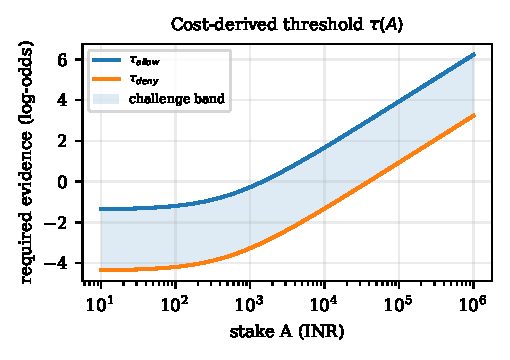
\includegraphics[width=\columnwidth]{figs/threshold.pdf}
\caption{Decision thresholds derived from Eqs.~\eqref{eq:tallow} and
\eqref{eq:tdeny}. The required evidence grows logarithmically with the stake;
the shaded region is where the system asks for re-verification instead of
committing.}
\label{fig:threshold}
\end{figure}

\subsection{Generalizing amount to stake}

An amount-only policy has a defect that is easy to miss: a request carrying no
monetary figure yields $A=0$ and therefore the \emph{lowest} threshold the
system can issue. ``Forward the one-time password'' and ``unlock the front
door'' would receive the cheapest verification in the system.

The Bayes rule needs $C_{\text{fa}}$, the cost of wrongly approving. A rupee
amount is one way to estimate that quantity, not its definition. We therefore
keep the derivation untouched and broaden the estimate:
\begin{equation}
\label{eq:stake}
A = \max\bigl(A_{\text{spoken}},\; A_{\text{consequence}},\; A_{\text{price}}\bigr),
\end{equation}
where $A_{\text{consequence}}$ is an anchor for the class of action and
$A_{\text{price}}$ is an estimate of the price of a named item. Because the
combination is a maximum, an \emph{under}estimate---the dangerous direction,
since $\tau$ increases with $A$---is absorbed by the anchor and changes
nothing, while an overestimate costs only friction. A fallible estimator can
therefore inconvenience a user but cannot open a hole.

The action class is assigned by a language model constrained to a fixed
enumeration and validated against it. The model never emits a currency figure
and never sees the anchor table; if it could name its own stake, an attacker
controlling the transcript would control the threshold. The anchors themselves
are declared policy constants, not measurements, and we treat them as
assumptions throughout.

Table~\ref{tab:stake} shows the effect. A request that toggles a lamp and a
request that discloses a one-time password differ by roughly seven units of
log-odds in the evidence they must clear, and both figures come from the same
formula.

\begin{table}[t]
\caption{Stake and resulting evidence requirement. Anchors are declared policy
constants, not measurements.}
\label{tab:stake}
\centering
\footnotesize
\begin{tabular}{@{}lrr@{}}
\toprule
\textbf{Request} & \textbf{Stake (INR)} & $\boldsymbol{\tau_{\text{allow}}}$ \\
\midrule
``What is the weather today?''      & 0       & $-1.38$ \\
``Turn off the lights.''            & 100     & $-1.19$ \\
``Order a packet of biscuits.''     & 1\,000  & $-0.28$ \\
``Transfer 10\,000 rupees.''        & 10\,000 & $1.67$ \\
``Buy a new laptop.''               & 350\,000 & $5.18$ \\
``Forward the one-time password.''  & 500\,000 & $5.53$ \\
\bottomrule
\end{tabular}
\end{table}

\subsection{The assistant as an attack surface}

Where a language model mediates the interaction, it is an attack surface rather
than an authority. We enforce one invariant: \emph{no language model output is
ever a verdict}. The model may emit features, which enter the decision only
after passing through the same calibration of Eq.~\eqref{eq:llr} as every other
layer, and it may verbalize a decision that has already been made. It cannot
produce an outcome, a threshold or an LLR. Every spoken response has a
deterministic template fallback, and a response contradicting the computed
decision is discarded in favour of that template.

\subsection{Decision procedure}

\begin{algorithmic}[1]
\STATE \textbf{Input:} audio $x$, enrolled centroid $\mathbf{c}$, history $H$
\STATE $T \leftarrow \mathrm{ASR}(x)$ \COMMENT{local, on-device}
\STATE $s_1 \leftarrow \cos(\mathbf{c}, \mathrm{embed}(x))$
\STATE $s_2 \leftarrow P(\text{playback}\mid x)$;\quad
       $s_3 \leftarrow P(\text{synthetic}\mid x)$
\STATE $s_4 \leftarrow \mathrm{context}(T, H)$
\STATE $A \leftarrow$ stake from $T$ by Eq.~\eqref{eq:stake}
\FOR{$\ell \in \{1,2,3,4\}$ with a score}
  \STATE $\Lambda_\ell \leftarrow \sigma(a_\ell s_\ell + b_\ell)$ mapped by Eq.~\eqref{eq:llr}
\ENDFOR
\STATE $\Lambda \leftarrow \min_\ell w_\ell \Lambda_\ell$
\STATE compute $\tau_{\text{allow}}(A), \tau_{\text{deny}}(A)$
\IF{$\Lambda \geq \tau_{\text{allow}}$} \RETURN ALLOW
\ELSIF{$\Lambda \geq \tau_{\text{deny}}$} \RETURN CHALLENGE
\ELSE \RETURN DENY
\ENDIF
\end{algorithmic}

A layer that produces no score is reported unavailable rather than silently
skipped or imputed as neutral, so that an audit record states which defences
were actually in play.

\section{Implementation Details}

The prototype is a FastAPI service with a browser front end. L1 uses the
SpeechBrain ECAPA-TDNN model \cite{ravanelli2021speechbrain} trained on
VoxCeleb. L3 uses AASIST-L \cite{jung2022aasist}, a raw-waveform graph
attention network of approximately $8.5\times10^{4}$ parameters operating on a
fixed 64\,600-sample (4.04\,s) window. L2 is a logistic model over spectral and
cepstral summary features. L4 combines an injection classifier, a
language-model extraction of social-engineering markers, and a behavioural
comparison against the user's own history; the three are multiplied as
independent ``nothing wrong here'' indicators.

Every authorization writes an audit record containing the user identifier,
timestamp, transcript, each layer's raw score and calibrated LLR, the derived
thresholds, the stake and its derivation, and the outcome. Because the
threshold is computed rather than looked up, the audit record is sufficient to
reconstruct any decision.

The CHALLENGE outcome is actioned rather than merely reported: the assistant
speaks, requests the enrolled passphrase, and the second utterance is scored by
the same layers. Text verification is a precondition---if the phrase does not
match, the challenge fails regardless of voice quality.

\section{Results and Discussion}

\subsection{Component baselines}

On ASVspoof 2019 logical access, AASIST-L reproduced its published performance
under our pipeline: $0.51\%$ equal error rate on the development set
(24\,844 utterances) and $\mathbf{0.99\%}$ on the evaluation set (71\,237
utterances), at approximately 67\,ms per utterance. An LFCC-GMM baseline
implemented for comparison reached $9.38\%$ development and $18.75\%$
evaluation EER. These are in-domain results and should be read as such.

A tandem experiment over 800 trials quantified the gap that motivates L3: the
speaker verification layer rejected $100\%$ of impostors but admitted $54.0\%$
of synthetic clones, of which L3 subsequently caught $87.0\%$ with no false
alarms on genuine trials.

\subsection{The domain gap}
\label{sec:domaingap}

Anti-spoofing performance is capture-dependent, and we observed this severely.
Genuine speech recorded through the browser was initially assigned
$P(\text{synthetic})=1.0$---the model's maximum confidence---while the same
speaker recorded on a phone scored $0.000$. The cause was the browser's default
signal processing. With echo cancellation, noise suppression and automatic gain
control disabled, false positives on 20 genuine browser-captured clips fell to
$1/20$, better than the phone reference ($2/8$). We report this because it is
an easily reproduced failure with an easily missed cause, and because it
supports a general rule: forensic audio layers must receive unprocessed
capture.

\subsection{Case study: the same utterance, spoken and replayed}

Table~\ref{tab:case} reports the per-layer evidence for one utterance spoken
live and then replayed through a loudspeaker and re-recorded on the same
microphone. It illustrates the argument for layering more directly than an
aggregate table can.

\begin{table}[t]
\caption{Per-layer calibrated evidence (LLR) for one utterance, spoken live
and replayed. L1 and L3 pass the replay, correctly.}
\label{tab:case}
\centering
\footnotesize
\begin{tabular}{@{}lrrl@{}}
\toprule
\textbf{Layer} & \textbf{Live} & \textbf{Replayed} & \textbf{Reading} \\
\midrule
L1 Voiceprint    & $+0.48$ & $+0.21$ & correct voice in both \\
L2 Liveness      & $+1.37$ & $\mathbf{-1.35}$ & only layer that objects \\
L3 Anti-spoofing & $+2.72$ & $+2.70$ & real vocal tract in both \\
L4 Context       & $+1.93$ & $+2.11$ & same benign request \\
\midrule
Fused (min)      & $+0.48$ & $-1.35$ & \\
\textbf{Outcome} & \textbf{ALLOW} & \textbf{CHALLENGE} & \\
\bottomrule
\end{tabular}
\end{table}

L1 and L3 do not fail on the replay; they succeed. The utterance genuinely is
the enrolled user's voice, and it genuinely was produced by a human vocal
tract. Under an additive rule their two correct positive statements would
outweigh L2's single correct negative one; under Eq.~\eqref{eq:fusion} the
objection stands.

\subsection{Layer ablation}
\label{sec:ablation}

Table~\ref{tab:ablation} and Fig.~\ref{fig:ablation} report false acceptance by
threat for layer subsets, over 400 composite trials per cell on held-out data.
Trials pair independently measured audio, liveness and command conditions; this
evaluates the fusion policy and assumes layer errors are independent, an
assumption a real deployment may violate.

\begin{table}[t]
\caption{False acceptance rate (\%) by threat, conjunctive fusion. Last column
is false rejection of genuine users. Bold marks the blindness created by
removing a layer.}
\label{tab:ablation}
\centering
\footnotesize
\setlength{\tabcolsep}{3.2pt}
\begin{tabular}{@{}lrrrrrr@{}}
\toprule
\textbf{Subset} & \textbf{Imp.} & \textbf{Replay} & \textbf{Clone} &
\textbf{Inj.} & \textbf{Soc.} & \textbf{FRR} \\
\midrule
L1 only            & 0.25 & \textbf{74.00} & \textbf{43.25} & \textbf{23.50} & \textbf{19.50} & 26.00 \\
L1+L3              & 0.25 & \textbf{74.00} & 1.50 & \textbf{23.50} & \textbf{19.50} & 26.00 \\
L1+L2+L3           & 0.25 & 1.25 & 1.50 & \textbf{23.50} & \textbf{19.50} & 27.00 \\
L1+L3+L4           & 0.25 & \textbf{62.00} & 1.25 & 10.00 & 7.25 & 38.00 \\
\textbf{All four}  & \textbf{0.25} & \textbf{1.25} & \textbf{1.25} & \textbf{10.00} & \textbf{7.25} & 38.75 \\
\bottomrule
\end{tabular}
\end{table}

\begin{figure}[t]
\centering
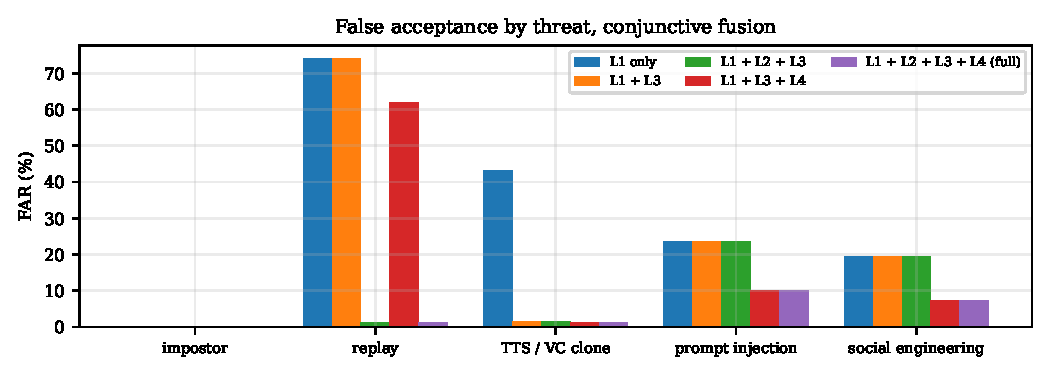
\includegraphics[width=\columnwidth]{figs/ablation.pdf}
\caption{False acceptance by threat for each layer subset. Every subset is
blind to at least one threat; the full system is best or tied-best in every
column.}
\label{fig:ablation}
\end{figure}

Every subset is blind to something, and the blindness is structural rather than
statistical. Removing L2 raises replay false acceptance from $1.25\%$ to
$74.0\%$, and the reason is visible in the per-layer evidence: for a replayed
utterance L1 and L3 both \emph{pass}, correctly, because it is genuinely the
enrolled user's voice and genuinely a human vocal tract. Only L2 objects.

The cost of the conjunctive rule is false rejection, which rises from $26.0\%$
to $38.75\%$ as layers are added. This figure should not be read as customers
turned away: of genuine users, $61.25\%$ are allowed immediately, $26.75\%$ are
challenged and recoverable through the spoken passphrase loop, and $12.0\%$ are
refused outright. This is what the three-outcome policy purchases, and it is
why $C_{\text{chal}} \ll C_{\text{rej}}$ in the cost model.

\subsection{Fusion rule comparison}

Fig.~\ref{fig:fusion} contrasts the two rules on the full system. Under
summation the ordering of subsets is non-monotonic and impostor false
acceptance is an order of magnitude worse. We report this as a negative result
about a standard technique applied to a non-standard structure.

\begin{figure}[t]
\centering
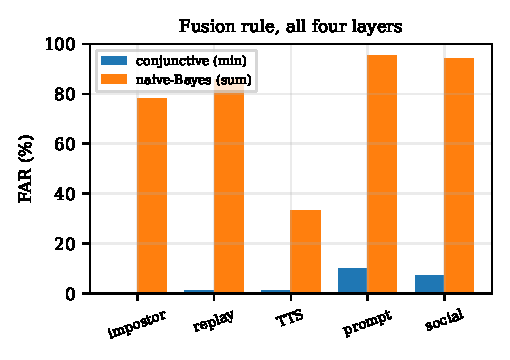
\includegraphics[width=0.92\columnwidth]{figs/fusion.pdf}
\caption{Conjunctive versus additive fusion, all four layers. Summation is
invalid here because the layers test different hypotheses.}
\label{fig:fusion}
\end{figure}

\subsection{Sensitivity to the assumed constants}
\label{sec:sensitivity}

The threshold's \emph{form} is derived, but its four constants
($C_h$, $C_{\text{chal}}$, $C_{\text{rej}}$, $\pi$) are assumptions, since we
have no fraud logs from which to estimate them. The material question is
therefore not whether they are correct but how wrong they can be before
behaviour changes. Fig.~\ref{fig:sensitivity} sweeps each over at least an
order of magnitude.

\begin{figure}[t]
\centering
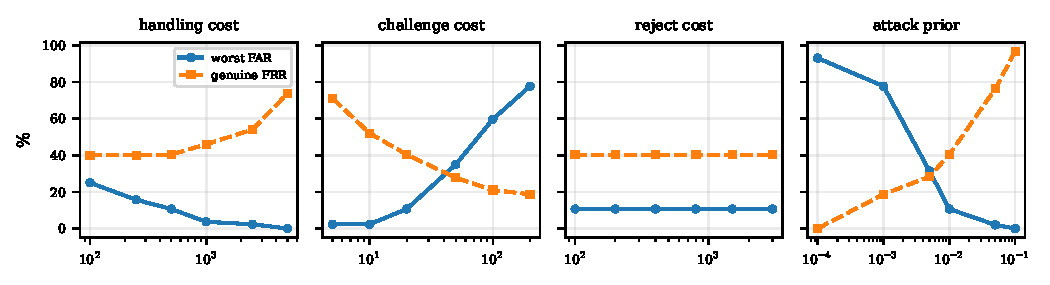
\includegraphics[width=\columnwidth]{figs/sensitivity.pdf}
\caption{Sensitivity of worst-case false acceptance and genuine false rejection
to each assumed constant. Dependence is concentrated in the attack prior.}
\label{fig:sensitivity}
\end{figure}

The result is informative and partly uncomfortable. Varying $C_{\text{rej}}$
changes which requests are challenged versus denied but leaves both FAR and FRR
unchanged, because it moves only the lower boundary. $C_h$ and
$C_{\text{chal}}$ behave as smooth, monotonic security-versus-friction dials.
The attack prior $\pi$, however, dominates: across the swept range, worst-case
FAR moves between $0.0\%$ and $93.0\%$ and genuine FRR between $0.0\%$ and
$96.7\%$.

We regard this as a useful localization rather than a refutation. Three of the
four constants are business policy and behave benignly; the one constant that
matters is the observed fraud rate, which is exactly the quantity a deployment
can estimate from its own logs. Our default $\pi=0.01$ is conservative relative
to typical transaction fraud rates, so error in this assumption biases the
system toward more verification rather than less.

\subsection{Liveness layer}

Under leave-one-pair-out cross-validation over 15 pairs, L2 achieved $100\%$
accuracy and $0\%$ EER. An identical figure from an earlier iteration of this
project proved to be an artefact---live clips were recorded on one device and
replays on another, so the classifier separated \emph{devices}. The present
corpus was captured so that each pair is recorded through one microphone
seconds apart, clips are cropped to a common length to remove a duration cue,
and 20 further genuine clips, unseen in training, were classified live at
$20/20$. The discriminating features are low-order cepstral means, consistent
with the spectral reshaping expected from an additional loudspeaker and room
path. \textbf{This result nevertheless rests on one speaker, one room and one
playback device---a laptop's built-in speakers, which are poor reproducers---and
must be validated against high-fidelity playback before it can be described as
a replay detector in general.}

\subsection{Comparison with the tiered baseline}

Table~\ref{tab:compare} contrasts the present design with the tiered
similarity-threshold scheme it replaces. The distinction we wish to draw is not
that one set of numbers is larger than another, but that the quantities in the
right-hand column are answerable: each is either measured, or is a stated
business assumption that a reviewer can dispute specifically.

\begin{table}[t]
\caption{Design comparison. The right column's parameters are auditable
quantities rather than score cutoffs.}
\label{tab:compare}
\centering
\footnotesize
\begin{tabular}{@{}p{1.7cm}p{2.5cm}p{2.9cm}@{}}
\toprule
 & \textbf{Tiered baseline} & \textbf{This work} \\
\midrule
Decision input & one cosine similarity & four calibrated LLRs \\
Threshold & fixed cutoffs (0.75 / 0.85) & derived, $\tau(A)$ \\
Amount handling & 3--4 hand-drawn bands & continuous, logarithmic \\
Non-monetary risk & not represented & stake, Eq.~\eqref{eq:stake} \\
Tunable numbers & score cutoffs & four business costs \\
Threats covered & impostor & impostor, replay, clone, manipulated request \\
Auditability & score and verdict & full derivation \\
\bottomrule
\end{tabular}
\end{table}

\section{Security, Privacy, and Limitations}

\subsection{Security properties}

The conjunctive rule of Eq.~\eqref{eq:fusion} gives a monotonicity guarantee:
adding a layer cannot increase $\Lambda$, so no new layer can admit an attack
that the previous configuration refused. Deriving the stake from speech does
not give an attacker leverage, because the stake sets only strictness; an
attacker who understates it to obtain a lower bar thereby restricts themselves
to a low-stake action. The language model's exclusion from the verdict path
means that a successful prompt injection can at most corrupt a feature, which
is then bounded by calibration, rather than dictate an outcome.

\subsection{Privacy}

Speech is biometric data. Transcription runs locally, and only text is exposed
to any external model, so raw audio does not leave the device. Voiceprints are
stored as 192-dimensional embeddings rather than audio. We note honestly that
embeddings are not anonymous---they identify the speaker by construction---and
that a deployment must treat them as sensitive personal data under the
applicable regime.

\subsection{Limitations}

\begin{enumerate}
\item \textbf{L4's corpus is template-generated.} No public corpus of labelled
adversarial voice-assistant commands exists. Reporting separation on this
corpus is legitimate; reporting its EER as a deployment estimate is not.
\item \textbf{L2 rests on 15 pairs}, one speaker, one room, one playback
device, as stated above.
\item \textbf{Composite trials assume independent layer errors.} No corpus
carries all conditions on one utterance. Correlated failures are plausible in
deployment.
\item \textbf{Live testing used a single speaker.} False rejection estimates
from it do not generalize; demographic bias is consequently unmeasured, and
speaker verification is known to exhibit performance disparities across
demographic groups.
\item \textbf{The stake anchors and cost constants are assumptions}, and the
action category is assigned by a language model, so category errors propagate
to the threshold.
\item \textbf{The passphrase is fixed}, so any recording of the user speaking
it satisfies the text check. A randomly chosen challenge phrase would remove
this weakness and is the natural next step.
\item \textbf{Voice conversion is under-tested} relative to text-to-speech, and
prior work reports that it is the harder attack family.
\end{enumerate}

\section{Conclusion and Future Work}

We presented an authorization architecture for voice assistants in which
heterogeneous detectors are calibrated to a common evidence scale, fused under
a rule appropriate to the fact that they test different hypotheses, and
compared against a threshold derived from the cost of being wrong about the
specific request. Measurement, rather than argument, established three results:
that additive fusion of calibrated scores is invalid in this setting and
degrades impostor detection by two orders of magnitude; that each of the four
evidence layers covers a threat the others structurally cannot, so that no
layer is redundant; and that the policy's dependence on its assumed constants
is concentrated almost entirely in the attack prior, which is the one constant
a deployment can measure.

Future work follows directly from the limitations. A randomly chosen challenge
phrase would give replay resistance independent of the acoustic liveness layer.
A larger and more diverse liveness corpus, including high-fidelity playback and
multiple speakers and rooms, is required before the liveness result can be
generalized. Collecting genuine adversarial commands, rather than templates,
would put L4 on the same evidentiary footing as L1 and L3. Estimating the
attack prior from deployment logs would convert the system's most sensitive
assumption into a measurement. Finally, a demographic evaluation is necessary
before any claim of fairness can be made.

\section*{Reproducibility}

All reported numbers are produced by scripts in the accompanying
implementation. Calibration uses development splits only; evaluation halves
were scored once. Random seeds are fixed and recorded alongside every result
file.

\begin{thebibliography}{00}

\bibitem{wu2015spoofing}
Z. Wu, N. Evans, T. Kinnunen, J. Yamagishi, F. Alegre, and H. Li,
``Spoofing and countermeasures for speaker verification: A survey,''
\emph{Speech Communication}, vol. 66, pp. 130--153, 2015.

\bibitem{todisco2019asvspoof}
M. Todisco \emph{et al.},
``ASVspoof 2019: Future horizons in spoofed and fake audio detection,''
in \emph{Proc. Interspeech}, 2019, pp. 1008--1012.

\bibitem{wang2020asvspoof}
X. Wang \emph{et al.},
``ASVspoof 2019: A large-scale public database of synthesized, converted and
replayed speech,'' \emph{Computer Speech \& Language}, vol. 64, 101114, 2020.

\bibitem{greshake2023injection}
K. Greshake, S. Abdelnabi, S. Mishra, C. Endres, T. Holz, and M. Fritz,
``Not what you've signed up for: Compromising real-world LLM-integrated
applications with indirect prompt injection,''
in \emph{Proc. ACM Workshop on Artificial Intelligence and Security (AISec)},
2023, pp. 79--90.

\bibitem{kinnunen2018tdcf}
T. Kinnunen, K. A. Lee, H. Delgado, N. Evans, M. Todisco, M. Sahidullah,
J. Yamagishi, and D. A. Reynolds,
``t-DCF: A detection cost function for the tandem assessment of spoofing
countermeasures and automatic speaker verification,''
in \emph{Proc. Odyssey: The Speaker and Language Recognition Workshop}, 2018,
pp. 312--319.

\bibitem{desplanques2020ecapa}
B. Desplanques, J. Thienpondt, and K. Demuynck,
``ECAPA-TDNN: Emphasized channel attention, propagation and aggregation in
TDNN based speaker verification,''
in \emph{Proc. Interspeech}, 2020, pp. 3830--3834.

\bibitem{ravanelli2021speechbrain}
M. Ravanelli \emph{et al.},
``SpeechBrain: A general-purpose speech toolkit,''
arXiv preprint arXiv:2106.04624, 2021.

\bibitem{nagrani2017voxceleb}
A. Nagrani, J. S. Chung, and A. Zisserman,
``VoxCeleb: A large-scale speaker identification dataset,''
in \emph{Proc. Interspeech}, 2017, pp. 2616--2620.

\bibitem{jung2022aasist}
J. Jung, H.-S. Heo, H. Tak, H.-J. Shim, J. S. Chung, B.-J. Lee, H.-J. Yu, and
N. Evans,
``AASIST: Audio anti-spoofing using integrated spectro-temporal graph attention
networks,'' in \emph{Proc. IEEE ICASSP}, 2022, pp. 6367--6371.

\bibitem{ravanelli2018sincnet}
M. Ravanelli and Y. Bengio,
``Speaker recognition from raw waveform with SincNet,''
in \emph{Proc. IEEE Spoken Language Technology Workshop (SLT)}, 2018,
pp. 1021--1028.

\bibitem{muller2022generalize}
N. M. M\"uller, P. Czempin, F. Dieckmann, A. Froghyar, and K. B\"ottinger,
``Does audio deepfake detection generalize?''
in \emph{Proc. Interspeech}, 2022, pp. 2783--2787.

\bibitem{ahmed2020void}
M. E. Ahmed, I.-Y. Kwak, J. H. Huh, I. Kim, T. Oh, and H. Kim,
``Void: A fast and light voice liveness detection system,''
in \emph{Proc. 29th USENIX Security Symposium}, 2020, pp. 2685--2702.

\bibitem{blue2022vocaltract}
L. Blue, K. Warren, H. Abdullah, C. Gibson, L. Vargas, J. O'Dell, K. Butler,
and P. Traynor,
``Who are you (I really wanna know)? Detecting audio deepfakes through vocal
tract reconstruction,''
in \emph{Proc. 31st USENIX Security Symposium}, 2022, pp. 2691--2708.

\bibitem{zhang2017dolphin}
G. Zhang, C. Yan, X. Ji, T. Zhang, T. Zhang, and W. Xu,
``DolphinAttack: Inaudible voice commands,''
in \emph{Proc. ACM SIGSAC Conf. on Computer and Communications Security (CCS)},
2017, pp. 103--117.

\bibitem{carlini2018audio}
N. Carlini and D. Wagner,
``Audio adversarial examples: Targeted attacks on speech-to-text,''
in \emph{Proc. IEEE Security and Privacy Workshops (SPW)}, 2018, pp. 1--7.

\bibitem{chen2021bob}
G. Chen, S. Chen, L. Fan, X. Du, Z. Zhao, F. Song, and Y. Liu,
``Who is real Bob? Adversarial attacks on speaker recognition systems,''
in \emph{Proc. IEEE Symposium on Security and Privacy (S\&P)}, 2021,
pp. 694--711.

\bibitem{cheng2022survey}
P. Cheng and U. Roedig,
``Personal voice assistant security and privacy---A survey,''
\emph{Proceedings of the IEEE}, vol. 110, no. 4, pp. 476--507, 2022.

\bibitem{platt1999probabilistic}
J. C. Platt,
``Probabilistic outputs for support vector machines and comparisons to
regularized likelihood methods,''
in \emph{Advances in Large Margin Classifiers}, MIT Press, 1999, pp. 61--74.

\bibitem{brummer2006application}
N. Br\"ummer and J. du Preez,
``Application-independent evaluation of speaker detection,''
\emph{Computer Speech \& Language}, vol. 20, no. 2--3, pp. 230--275, 2006.

\bibitem{kinnunen2020tandem}
T. Kinnunen, H. Delgado, N. Evans, K. A. Lee, V. Vestman, A. Nautsch,
M. Todisco, X. Wang, M. Sahidullah, J. Yamagishi, and D. A. Reynolds,
``Tandem assessment of spoofing countermeasures and automatic speaker
verification: Fundamentals,''
\emph{IEEE/ACM Trans. Audio, Speech, and Language Processing}, vol. 28,
pp. 2195--2210, 2020.

\bibitem{radford2023whisper}
A. Radford, J. W. Kim, T. Xu, G. Brockman, C. McLeavey, and I. Sutskever,
``Robust speech recognition via large-scale weak supervision,''
in \emph{Proc. International Conference on Machine Learning (ICML)}, 2023,
pp. 28492--28518.

\bibitem{yamagishi2021asvspoof}
J. Yamagishi \emph{et al.},
``ASVspoof 2021: Accelerating progress in spoofed and deepfake speech
detection,'' in \emph{Proc. ASVspoof Workshop}, 2021, pp. 47--54.

\bibitem{tak2021rawnet}
H. Tak, J. Patino, M. Todisco, A. Nautsch, N. Evans, and A. Larcher,
``End-to-end anti-spoofing with RawNet2,''
in \emph{Proc. IEEE ICASSP}, 2021, pp. 6369--6373.

\end{thebibliography}

\end{document}
